\chapter{The First Chapter}\label{chap:first}

This is a newer and tastier version of the ECTE45x thesis style. It is more
compact with less space between title and text, equations and text, and the
reference list is smaller and more compact. 

The first chapter is obviously Chapter number~\ref{chap:first}. I am now
citing \citet{RN6}, \citet{RN6} and EPRI \citep{RN6}.
BibTeX will take care of the entries for me.  Blah blah \ldots In this case,
the bibliography file is expected to be called `thesis.bib'.

Go on and describe contents of chapter, blah blah blah \ldots

\section{First Section in Chapter}\label{first:sec}

This is section~\ref{first:sec}.

\section{Another Section in Chapter}

Figure~\ref{fig:example} is an example of a figure containing an image.
Blah blah \ldots

\begin{figure}[!h]
\begin{singlespace}
\centering
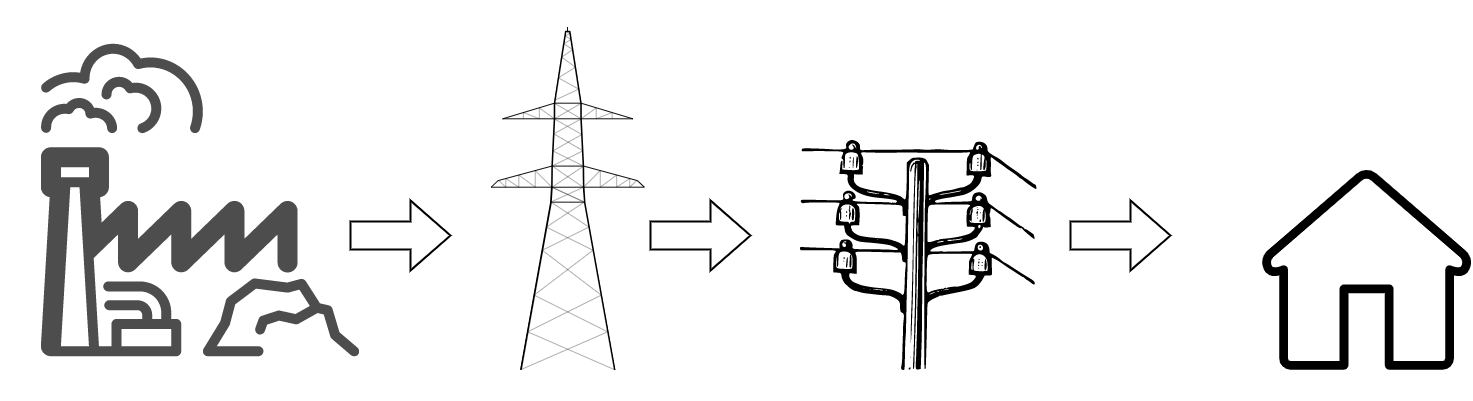
\includegraphics[width=8cm]{ElectricalGrid.png}
\caption[Caption for the List of Figures.]{Caption for the text body. We can
make this one really really long in order to describe everything
about the figure for which this caption references, noting that
the caption for the index really should be much shorter.}
\label{fig:example}
\end{singlespace}
\end{figure}

\subsection{First Subsection}

This is the first subsection in this report. Notice how the title has been
formatted as one would expect. Try doing that with other, inferior products.

\subsubsection{First Subsubsection}

This is the first subsubsection. You wouldn't want to descend much further
than this. Subsubsections are not numbered and do not appear in the table of
contents.

\section{Summary}

Blah blah \ldots

And now for some handy math hints via equation examples:
\begin{equation}
A=\frac{1}{\displaystyle\sum_{k=1}^{}}
\end{equation}
\begin{equation}
A=n^{\frac{1}{3}}
\end{equation}
\begin{equation}
A=n^{\frac{1}{3}}\max_{k=1}
\end{equation}
